\documentclass{article} % For LaTeX2e
\usepackage{nips14submit_e,times}
\usepackage{amsmath}
\usepackage{amsthm}
\usepackage{amssymb}
\usepackage{mathtools}
\usepackage{hyperref}
\usepackage{url}
\usepackage{algorithm}
\usepackage[noend]{algpseudocode}
%\documentstyle[nips14submit_09,times,art10]{article} % For LaTeX 2.09

\usepackage{bbm}
\usepackage{graphicx}
\usepackage{caption}
\usepackage{subcaption}
\usepackage{MnSymbol}

\def\eQb#1\eQe{\begin{eqnarray*}#1\end{eqnarray*}}
\def\eQnb#1\eQne{\begin{eqnarray}#1\end{eqnarray}}
\providecommand{\e}[1]{\ensuremath{\times 10^{#1}}}
\providecommand{\pb}[0]{\pagebreak}
\DeclarePairedDelimiter\ceil{\lceil}{\rceil}
\DeclarePairedDelimiter\floor{\lfloor}{\rfloor}

\newcommand{\E}{\mathrm{E}}
\newcommand{\Var}{\mathrm{Var}}
\newcommand{\Cov}{\mathrm{Cov}}
\newcommand\eqD{\stackrel{\mathclap{\normalfont\mbox{d}}}{=}}

\def\Qb#1\Qe{\begin{question}#1\end{question}}
\def\Sb#1\Se{\begin{solution}#1\end{solution}}

\newenvironment{claim}[1]{\par\noindent\underline{Claim:}\space#1}{}
\newtheoremstyle{quest}{\topsep}{\topsep}{}{}{\bfseries}{}{ }{\thmname{#1}\thmnote{ #3}.}
\theoremstyle{quest}
\newtheorem*{definition}{Definition}
\newtheorem*{theorem}{Theorem}
\newtheorem*{lemma}{Lemma}
\newtheorem*{question}{Question}
\newtheorem*{preposition}{Preposition}
\newtheorem*{exercise}{Exercise}
\newtheorem*{challengeproblem}{Challenge Problem}
\newtheorem*{solution}{Solution}
\newtheorem*{remark}{Remark}
\usepackage{verbatimbox}
\usepackage{listings}
\usepackage{mathrsfs}
\title{ProbLimI: \\
Problem Set VIII}


\author{
Youngduck Choi \\
CIMS \\
New York University\\
\texttt{yc1104@nyu.edu} \\
}


% The \author macro works with any number of authors. There are two commands
% used to separate the names and addresses of multiple authors: \And and \AND.
%
% Using \And between authors leaves it to \LaTeX{} to determine where to break
% the lines. Using \AND forces a linebreak at that point. So, if \LaTeX{}
% puts 3 of 4 authors names on the first line, and the last on the second
% line, try using \AND instead of \And before the third author name.

\newcommand{\fix}{\marginpar{FIX}}
\newcommand{\new}{\marginpar{NEW}}

\nipsfinalcopy % Uncomment for camera-ready version

\begin{document}


\maketitle

\begin{abstract}
This work contains solutions to the exercises of the problem set VIII. The
chosen problems are 1,2, and 3.
\end{abstract}

\bigskip

\begin{question}[1]
\hfill
\begin{figure}[h!]
  \centering
    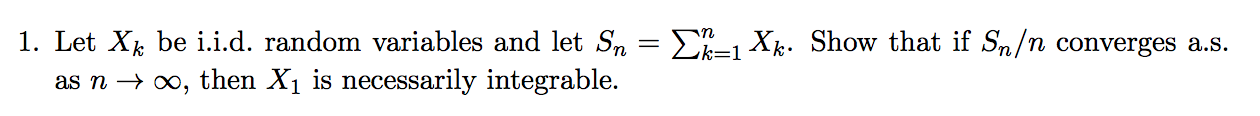
\includegraphics[width=0.7\textwidth]{prob-e8-p1.png}
\end{figure}
\end{question}
\begin{solution} \hfill \\
Suppose for sake of contradiction that $\mathbb{E}|X_1| = \infty$.
By Tonelli,
\eQb
\mathbb{E}|X_1| &=& \int_{\Omega} |X_1| d\mathbb{P} = \int_{\Omega} \int_{0}^{|X_1|} 
1 dy d\mathbb{P} = \int_{\Omega} \int_{0}^{\infty} 1_{\{ |X_1| > y\}} dy d\mathbb{P} \\
&=& \int_{0}^{\infty} \int_{\Omega} 1_{\{|X_1| > y\}} \mathbb{P} dy 
= \int_{0}^{\infty} \mathbb{P}(|X_1| > y) dy.  
\label{eq: 1-1} \eQe
Since
\eQb
\int_{0}^{n}\mathbb{P}(|X_1| > y) \leq \sum_{k=0}^{n} \mathbb{P}(|X_1| > k) 
\eQe
for all $n \geq 1$, from \eqref{eq: 1-1}, 
\eQb
\sum_{k=0}^{\infty} \mathbb{P}(|X_1| > k) = \infty. 
\eQe
Therefore, by Borel Cantelli II, 
\eQb
\mathbb{P}(|X_n| \geq n \>\> \text{i.o.}) &=& 1. 
\eQe
Now, observe that
\eQb
\dfrac{S_n}{n} - \dfrac{S_{n+1}}{n+1} &=& \dfrac{S_n}{n(n+1)} - \dfrac{X_{n+1}}{n+1}
\eQe
and hence, by reverse triangle inequality,
\eQb
|\dfrac{S_n}{n} - \dfrac{S_{n+1}}{n+1}| &\geq& 
||\dfrac{S_n}{n(n+1)}| - |\dfrac{X_{n+1}}{n+1}||
\eQe
for all $n \geq 1$. Suppose 
\eQb
w \in \{ \dfrac{S_n}{n} \>\>\> \text{converges}\} \cap \{|X_n| \geq n \>\> \text{i.o}\}. 
\eQe
Then, by the convergence of $\dfrac{S_n(w)}{n}$, 
there exists $0 < \delta < 1$ such that 
\eQb
|\dfrac{S_n(w)}{n(n+1)}| < \delta 
\eQe
for all $n$ large enough, and hence 
\eQb
|\dfrac{S_n(w)}{n} - \dfrac{S_{n+1}(w)}{n+1}| &>& 1 - \delta \>\>\> \text{i.o.}, 
\eQe
which contradicts the fact that $\dfrac{S_n(w)}{n}$ converges. Hence,
\eQb
\{ \dfrac{S_n}{n} \>\>\> \text{converges}\} \cap \{|X_n| \geq n \>\> \text{i.o}\} 
= \emptyset 
\eQe
so
\eQb
\mathbb{P}(\dfrac{S_n}{n} \>\>\> \text{converges}) &=& 0 
\eQe
which contradicts that $\dfrac{S_n}{n}$ converges a.s. 
Hence, $\mathbb{E}|X_1| < \infty$, i.e. $X_1$ is integrable. \hfill $\qed$
 
\end{solution}

\newpage

\begin{question}[2]
\hfill
\begin{figure}[h!]
  \centering
    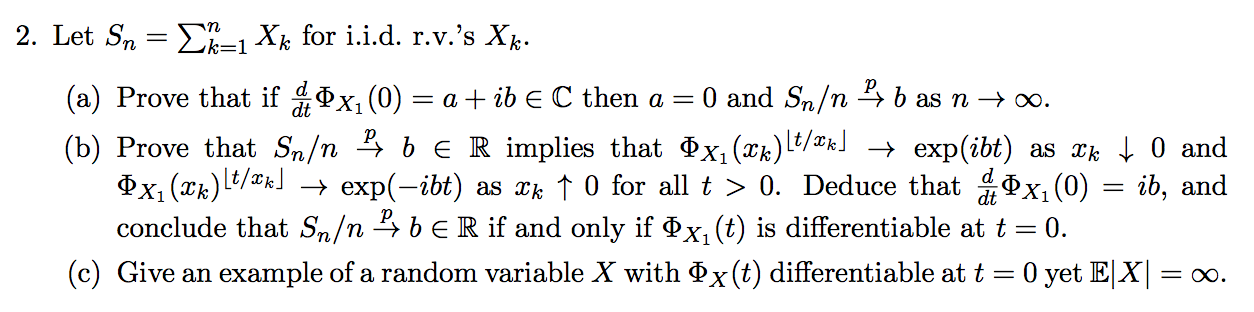
\includegraphics[width=0.7\textwidth]{prob-e8-p2.png}
\end{figure}
\end{question}
\begin{solution} \hfill \\
\textbf{(a)} Let $\dfrac{d}{dt} \Phi_{X_1}(0) = a + ib$. Then, there exists
$t_0>0$ small enough such that
\eQnb
\Phi_{X_1}(t_0) = 1 + (a+ib)t_0 + o(|t_0|) \>\>\> &\text{and}&
\Phi_{X_1}(-t_0) = 1 - (a+ib)t_0 + o(|t_0|).
\label{eq:2.22} \eQne

As $\Phi_{X_1}(t) = 
\overline{\Phi_{X_1}(-t)}$ for any $t \in \mathbb{R}$, from~\eqref{eq:2.22},
\eQb
(1+ at_0) + bt_0 i &=& (1-a t_0) + bt_0 i 
\eQe
which implies $a = 0$. Observe that
\eQb
\Phi_{n^{-1}S_n}(t) &=& \Phi_{X_1}(\dfrac{t}{n})^n = (1 + \dfrac{bti}{n} + o(\dfrac{
1}{n}))^n  
\eQe
for any $t \in \mathbb{R}$ and $n \in \mathbb{N}$. Taking $n \to \infty$, we see
that
\eQb
\Phi_{n^{-1}S_n}(t) &=& e^{ibt} 
\eQe
so by continuity theorem, $\dfrac{S_n}{n} \to_{D} b$ as $n \to \infty$. From pset 4-1,
$\dfrac{S_n}{n} \to_{p} b$ to $n \to \infty$.

\bigskip

\textbf{(b)} 
Since convergence in probability implies convergence in distribution, and by 
continuity theorem,
\eQb
\Phi_{X_1}(\dfrac{t}{n})^n \to e^{ibt}
\eQe
for all $t \in \mathbb{R}$. Let $t \in \mathbb{R}$, and $\epsilon > 0$. By 
uniform continuity of $\Phi_{X_1}$, there exists $ \delta > 0$,
\eQb
|\dfrac{t}{n_k} - x_k| < \delta &\implies& |\Phi_{X_1}(x_k) - \Phi_{X_1}(\dfrac{t}{
n_k})| < \epsilon.
\eQe 
where $\{n_k\}$ is any subsequence of $\{n\}$. Since $x_k \to 0$ and $n_k \to \infty$,
\eQb
|\Phi_{X_1}(x_k) - \Phi_{X_1}(\dfrac{t}{n_k})| < \epsilon
\eQe
and
\eQb
(\Phi_{X_1}(\dfrac{t}{n_k}) - \epsilon)^{n_k - n_k + \lfloor \frac{t}{x_k} \rfloor} 
&\leq& \Phi_{X_1}(x_k)^{\lfloor \frac{t}{x_k} \rfloor}  
\leq
(\Phi_{X_1}(+\dfrac{t}{n_k}) + \epsilon)^{n_k - n_k + \lfloor \frac{t}{x_k} \rfloor} 
\eQe 
for all $k$ large enough. Since $\epsilon > 0$ was arbitrary, we can take $\{\epsilon_k\}
$ such that $\epsilon_k \to 0$. Then, by the givens,
\eQb
\Phi_{X_1}(x_k)^{\lfloor \frac{t}{x_k} \rfloor} \to e^{ibt} 
\eQe 
as $k \to \infty$.
For the negative part, consider the conjugate relation as part a, then
carry out the exact same limit process.

\bigskip

To conclude, conversely, suppose $\Phi(\dfrac{t}{n})^n \to e^{ibt}$, then by taking logs 
$n\log(\Phi(\dfrac{t}{n})) \to ibt$. By differenability of $\log(z)$ for $z=1$
on the complex plane, $n(\Phi(\dfrac{t}{n}) - 1) \to ibt$. Hence, by the above
result and $(a)$, we have that $\Phi(t)$ is differentiable at $t =0$. 

\bigskip

\textbf{(c)} Define each $X$ such that
\eQb
\mathbb{P}(X = (-1)^k k) = C\dfrac{k}{k^2 \log(k)} 
\eQe
for all $k \geq 2$, where $C$ is the normalization constant. Then,
\eQb
\mathbb{E}|X| &=& \sum_{k=2}^{\infty} \dfrac{C}{k\log(k)} = \infty. 
\eQe
Furthermore,
\eQb
n\mathbb{P}(|X|>n) &=& n\sum_{k=n+1}^{\infty} \dfrac{C}{k^2 \log(k)} \to 0
\eQe
and 
\eQb
\mathbb{E}(X1_{\{|X|\leq n\}}) = \sum_{k=2}^{n} (-1)^k \dfrac{C}{k\log(k)} \>\>\>
\text{converges} 
\eQe
as $n \to \infty$. Hence, from thm 2.2.7 in Durrett,
\eQb
\dfrac{S_n}{n} \to_{P} \sum_{k=2}^{\infty} (-1)^k \dfrac{C}{k\log(k)} 
\eQe
and by $(b)$, $\Phi_{X}$ is differentiable at $t = 0$. Therefore, $X$ 
is the desired construction. 
\hfill $\qed$

\end{solution}

\newpage

\begin{question}[4]
\hfill
\begin{figure}[h!]
  \centering
    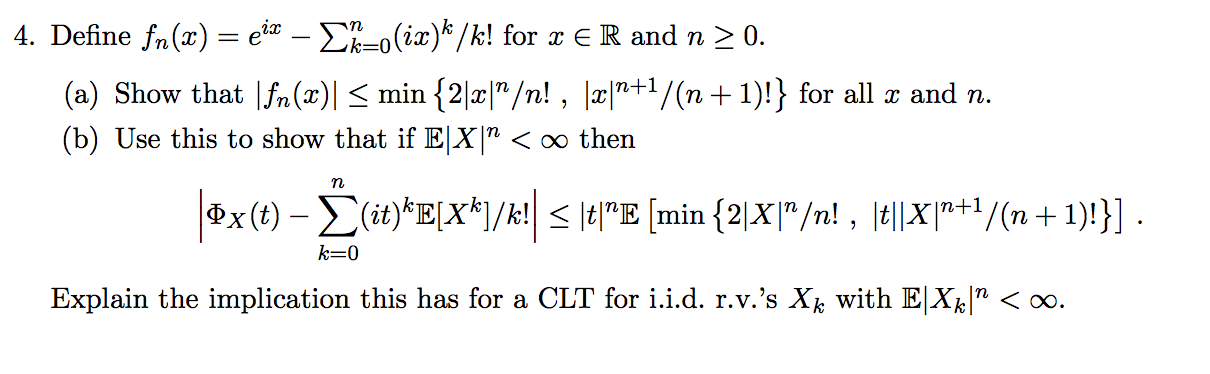
\includegraphics[width=0.7\textwidth]{prob-e8-p4.png}
\end{figure}
\end{question}
\begin{solution} \hfill \\
Let $x \in \mathbb{R}$. By integration by parts,
\eQnb 
\int_{0}^{x} (x-s)^n e^{is} ds &=& \dfrac{x^{n+1}}{n+1} + \dfrac{i}{n+1}
\int_{0}^{x} (x-s)^{n+1}e^{is} ds
\label{eq:4} \eQne 
for each $n \geq 0$. If $n = 0$, then
\eQb
x + i \int_{0}^{x} (x-s)e^{is} ds &=& \int_{0}^{x} e^{is}ds = \dfrac{e^{ix} - 1}{i} 
\eQe
and hence
\eQb
e^{ix} = 1 + ix + i^{2} \int_{0}^{x} (x-s)e^{is} ds. 
\eQe
Suppose for some $n > 0$
\eQnb
e^{ix} - \sum_{k=0}^{n} \dfrac{(ix)^k}{k!} &=& \dfrac{i^{n+1}}{n!} \int_{0}^{x}
(x-s)^n e^{is} ds  
\label{eq:4.1}
\eQne

Then, combined with~\eqref{eq:4},
\eQb
e^{ix} - \sum_{k=0}^{n+1} \dfrac{(ix)^{k}}{k!} 
&=& \dfrac{i^{n+1}}{n!} \int_{0}^{x} (x-s)^n e^{is} ds - \dfrac{(ix)^{n+1}}{(n+1)!} \\
&=& \dfrac{i^{n+1}}{n!}(\int_{0}^{x} (x-s)^n e^{is} ds - \dfrac{x^{n+1}}{(n+1)} \\
&=& \dfrac{i^{n+2}}{(n+1)!} \int_{0}^{x} (x-s)^{n+1} e^{is} ds. 
\eQe
Hence, by induction,~\eqref{eq:4.1} holds for all $n \geq 0$. If  $x \geq 0$, then
\eQb
|\dfrac{i^{n+1}}{n!} \int_{0}^{x} (x-s)^n e^{is} ds| &\leq&
\dfrac{1}{n!} \int_{0}^{x} |(x-s)^n| ds = \dfrac{1}{n!} \int_{0}^{x} 
(x-s)^n ds = \dfrac{1}{(n+1)!} |x|^{n+1}.
\eQe
If $x < 0$, then
\eQb
|\dfrac{i^{n+1}}{n!} \int_{0}^{x} (x-s)^n e^{is} ds| &=&
|\dfrac{i^{n+1}}{n!} \int_{x}^{0} (x-s)^n e^{is} ds|
\leq
\dfrac{1}{n!} \int_{x}^{0} |(x-s)^n e^{is}| ds \\
&\leq&
\dfrac{1}{n!} \int_{x}^{0} (s-x)^n  ds = \dfrac{1}{(n+1)!} (-x)^{n+1} 
= \dfrac{1}{(n+1)!}|x|^{n+1}.
\eQe
Therefore,
\eQnb
|f_n(x)| &\leq& \dfrac{1}{(n+1)!} |x|^{n+1} 
\label{eq:4.2} \eQne
for any $n \geq 0$. Now, again by integration by parts,
\eQb
\dfrac{i}{n} \int_{0}^{x} (x-s)^{n} e^{is} ds &=& -\dfrac{x^n}{n} + \int_{0}^{x}
(x-s)^{n-1} e^{is} ds 
\eQe
and hence
\eQb
\dfrac{i^{n+1}}{n!} \int_{0}^{x} (x-s)^{n} e^{is} ds = \dfrac{i^n}{(n-1)!}
\int_{0}^{x} (x-s)^{n-1}(e^{is} - 1) ds
\eQe
for any $n \geq 1$. If $x \geq 0$, then
\eQb
|\dfrac{i^{n+1}}{n!} \int_{0}^{x} (x-s)^{n} e^{is} ds| &=& |\dfrac{i^n}{(n-1)!} 
\int_{0}^{x} (x-s)^{n-1} (e^{is}  - 1) ds| \\
&\leq& \dfrac{1}{(n-1)!} \int_{0}^{x} |(x-s)^{n-1}||e^{is} - 1| ds \\
&\leq& \dfrac{2}{(n-1)!} \int_{0}^{x} (x-s)^{n-1} ds = \dfrac{2}{n!} |x|^{n}. 
\eQe
If $ x < 0$, then
\eQb
|\dfrac{i^{n+1}}{n!} \int_{0}^{x} (x-s)^{n} e^{is} ds| &=& |\dfrac{i^n}{(n-1)!} 
\int_{0}^{x} (x-s)^{n-1} (e^{is}  - 1) ds| \\
&\leq& \dfrac{1}{(n-1)!} \int_{0}^{x} |(x-s)^{n-1}||e^{is} - 1| ds \\
&\leq& \dfrac{2}{(n-1)!} \int_{0}^{x} (x-s)^{n-1} ds = \dfrac{2}{n!} |x|^{n}. 
\eQe
Therefore, combined with ~\eqref{eq:4.2}, 
\eQb
|f_n(x)| &\leq& \min(\dfrac{2|x|^n}{n!}, \dfrac{|x|^{n+1}}{(n+1)!}) 
\eQe
for all $x \in \mathbb{R}$ and $n \geq 1$. 

\bigskip

\textbf{(ii)} From the above estimate,
\eQb
|e^{itX} - \sum_{k=0}^{n} \dfrac{(itX)^k}{k!}| &\leq& 
\min(\dfrac{2|tX|^{n}}{n!}, \dfrac{|tX|^{n+1}}{(n+1)!}) \\
\eQe
and hence, by Jensen's inequality, and 
linearity of expectation, which is granted by $\mathbb{E}|X|^n < \infty$,
\eQb
|\Phi_{X}(t) - \sum_{k=0}^{n} \dfrac{\mathbb{E}(itX)^k}{k!}| &\leq& 
\mathbb{E}|e^{itX} - \sum_{k=0}^{n} \dfrac{(itX)^k}{k!}| \\ &\leq&
\mathbb{E}\left[ \min(\dfrac{2|tX|^{n}}{n!}, \dfrac{|tX|^{n+1}}{(n+1)!})\right] \\
&=& |t|^n 
\mathbb{E}\left[ \min(\dfrac{2|X|^{n}}{n!}, \dfrac{|t||X|^{n+1}}{(n+1)!})\right] \\
\eQe
for all $t \in \mathbb{R}$.

\bigskip


Suppose $\mathbb{E}|X|^2 < \infty$. Let $t \in \mathbb{R}$. Then,
\eQb
\Phi_{X}(t) &=& 1 + it\mathbb{E}X - t^2\mathbb{E}\dfrac{X^2}{2} + \Psi(t)
\eQe  
for some constant $\Psi$, dependent on $t$.
By the established result,
\eQb
|\Psi(t)| &\leq& t^2 \mathbb{E}(|t||X|^3 \wedge 2|X|^2) 
\eQe
where denotes the minimum operation. Observe that as $t \to 0$,
\eQb
|t||X|^3 \wedge 2|X|^2  \to 0 \>\> \text{everywhere} \>\>\> \text{and} \>\>\>
|t||X|^3 \wedge 2|X|^2 \leq 2|X|^2 \text{everywhere}. 
\eQe
Since $\mathbb{E}|X|^2 < \infty$, by DCT,
\eQb
\dfrac{|\Psi(t)|}{t^2} \to 0 
\eQe
so 
\eQb
\Phi_{X}(t) &=& 1 + it\mathbb{E}X - t^2\mathbb{E}\dfrac{X^2}{2} + o(t^2).
\eQe
This shows that we can prove the CLT for the iid case without assuming the finite
third moment. \hfill $\qed$
\end{solution}


\end{document}
